\chapter{Problem statement and proposal}\label{B:problemStatementAndProposal}

The goal of this chapter is to provide a structured vision of the specific problems of each one of the points to be developed within this thesis.

The main challenges are to prepare and/or adapt current technologies to be ready for a cloud deployment. This fact implies studying the existing technologies and tools in order to create specific services that will be interconnected between them. Finally, the required developments will be carried out in order to assure the goals behind and ease demonstrate the results.

The main goals of this thesis are:

\begin{itemize}
\item To implement a high-level HTTP REST API in order to manage and monitor the LiveMediaStreamer framework.
\item To demonstrate that LMS is able to be deployed in a virtualized environment.
\item To enhance LMS with specific metrics measurements in order to demonstrate its capabilities as a real-time media streaming framework.
\item To offer a set of tools which gather the aforementioned metrics and present them in order to demonstrate the previous statements.
\item To include all previous statements within an architecture proposal.
\item To demonstrate previous statements in specific testing deployments.
\end{itemize}

\section{Architecture analysis}

The main requirement is to define the platform's architecture to be prototyped in order to have a global and generic insight. So, taking into account the pieces required for this thesis (i.e.: service layer, monitoring layer, virtualization/deployment layer), such architecture should contain the different high level layers as shown in Figure \ref{F:genericPlatArch}.
\begin{figure}[htb]
\begin{center}
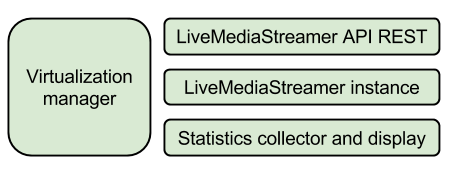
\includegraphics[width=0.6\textwidth]{./images/generalArch.png}
\caption{Generic platform architecture}
\label{F:genericPlatArch}
\end{center}
\end{figure}

The "LiveMediaStreamer REST API" layer will contain the service that will be offered to different and external applications (communicating over HTTP) in order to manage the "LiveMediaStreamer instance" layer by creating different audio and video production scenarios. Both layers are the core layers of the platform. 

Moreover, in order to offer a centralized monitoring system, the "Statistics collector and display" layer becomes as the generic box for this requirement.

It is also required to provide an orchestrator that manages the deployment and distribution of the possible configurations for the previous introduced layers. This will be done thanks to the "Virtualization manager" layer.

Finally, an important point is to define how the communication between each layer is going to be carried out. This is described in the following sections.

\subsection{Virtualization}

This subsection aims to introduce the possibilities that different virtualization technologies can offer in our project requirements, and to decide between one of them.

First of all, the following points show which are the expected outcomes for using virtualization and what requirements should the selected technology fulfill:

\begin{itemize}
\item To manage and maintain a system of small pieces of services
\item To have flexibility in order to quickly instantiate (e.g.: start, restart, stop) the required instances (e.g.: to assure real-time scalability) and to deploy any possible required scenario/configuration
\item To offer ease of continuous development and deployment of the different parts of the architecture
\item To have a virtualizatied application version control system for having different version tags for the architecture modules (e.g.: a development and a production container of the same REST API service)
\item To assure full compatibility for the core layers' operating system (right now only Linux environments are supported)
\item To assure full compatibility for the hardware to work with (mainly x86 processors are in the scope)
\end{itemize}

Moreover, it is also required to use a technology that is as much lightweight as possible. Since we want to virtualize each piece of the platform architecture.

Under Linux environments there are many virtualization options to analyse (most of them proprietary), but let us focus on the ones that are open-source and have wider and active communities behind. These are:

\begin{itemize}
\item KVM (Kernel-based Virtual Machines) \cite{kvm}\hfill

It is a FreeBSD and Linux kernel module that offers a full virtualization solution for Linux on x86 hardware containing virtualization extensions (Intel VT or AMD-V). It consists of a loadable kernel module that provides the core virtualization infrastructure and a processor specific module.
Usually, KVM runs with the QEMU (Quick Emulator) \cite{qemu} which is a complete and standalone emulation suite that performs hardware virtualization.

KVM with QEMU are able to offer virtualization for x86, PowerPC, and S/390 guests. For instance, when the target architecture is the same as the host architecture, QEMU can make use of KVM particular features in order to not emulate CPU nor memory by using the offered by the host kernel.

\begin{figure}[!htb]
\begin{center}
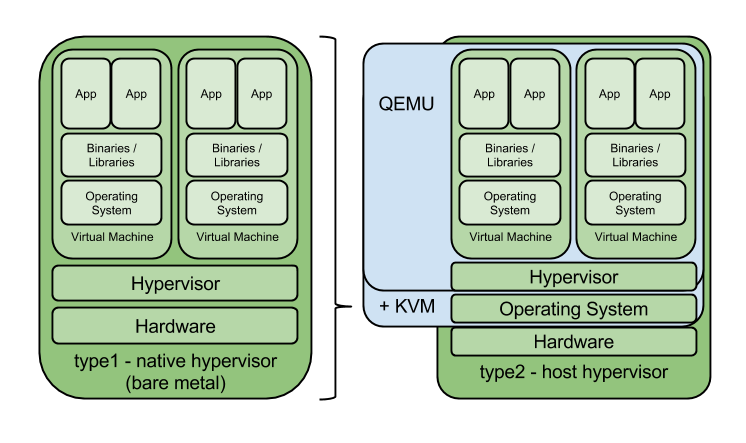
\includegraphics[width=0.9\textwidth]{./images/KVM.png}
\caption{QEMU with KVM or hypervisor type2 to type1}
\label{F:KVMandQEMU}
\end{center}
\end{figure}

Figure \ref{F:KVMandQEMU} showcases how KVM can convert a type2 hypervisor (i.e.: QEMU) into a type1 hypervisor (known as a bare metal hypervisor) which increases overall application performances. 

\item LXC (Linux Containers) \cite{lxc}\hfill

It is an operating-system-level virtualization environment able to run multiple isolated Linux systems (known as containers) on a single Linux central host.

Linux kernel itself provides the cgroups functionality that allows limitation and prioritization of resources (CPU, memory, block I/O, network, etc.) without the need for starting any virtual machines, and namespace isolation functionality that allows complete isolation of an applications' view of the operating environment, including process trees, networking, user IDs and mounted file systems.

Nowadays virtualization tendencies are focusing on the Docker project \cite{docker}, which is a platform that provides an additional layer of abstraction and automation of operating-system-level virtualization on Linux, Mac OS and Windows.
\begin{figure}[!htb]
\begin{center}
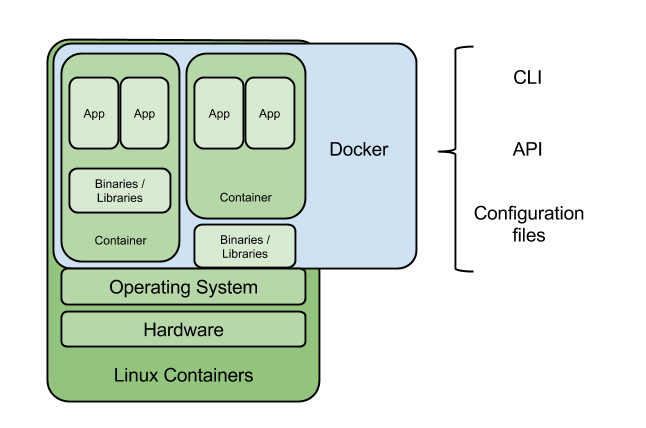
\includegraphics[width=0.9\textwidth]{./images/LXC.png}
\caption{Docker with LXC}
\label{F:DockerAndLXC}
\end{center}
\end{figure}

Using LXC with Docker mean resource isolation to allow independent containers to run within a single Linux instance, avoiding the overhead of starting and maintaining virtual machines. Moreover, the Docker project automates the deployment of applications inside software containers and offers different tools to manage them (i.e.: CLI, API and file configurations), as shown in Figure \ref{F:DockerAndLXC}. 
\end{itemize}

Thus, it seems that the technology that best suits this thesis requirements is the Docker project. The main reasons are the capabilities of ease maintenance, test and quickly deploy each container. 

Finally, it is important to point out that another key feature of the Docker solution is that it allows containers to intercommunicate containers that are in the same physical server by isolating its network layer. This means much more security and performance over other virtualization solutions (at least of the simplicity point of view when intercommunicating instances).

\subsection{Monitoring layer}

We now provide an insight on the minimum requirements for the monitoring module, together with an analysis of available tools. Following the same criteria used previously, we focus on open-source tools. 

The main requirements for the monitoring layer implementation are:

\begin{itemize}
\item To ease distributed deployments.
\item To offer full control for specific configuration requirements and to not depend on external/enterprise services. 
\item To be fully deployable.
\item To be as lightweight as possible in terms of:
\begin{itemize}
\item Processing capacity
\item Memory utilization
\item Network throughput
\end{itemize}
\item To be supported under a Linux environment.
\item To be flexible and scalable enough to be used in future extensions of the project.
\item To support RRD (Round Robin Database) as a DBMS (Database Management System) in order to control data storage size.
\end{itemize}

The data to be gathered includes:

\begin{itemize}
\item CPU and memory usage per process.
\item Network usage (per process involved and per media flow)
\item Internal core service performance parameters (i.e.: LiveMediaStreamer core performance):
\begin{itemize}
\item Processing time
\item Data block losses ratio
\end{itemize}
\end{itemize}

We propose to split the monitoring layer in order to ensure stated requirements. The proposal, as usually done in many monitoring tools such as system monitoring, follows this model:
\begin{itemize}
\item Gathering layer \hfill

It will only be responsible of the gathering, distribution and storing of the metrics.

\item Display layer

It will only be responsible of displaying data in answer of user-specific queries.

\end{itemize}
An alert layer could be considered as a future development. This thesis is focused on measuring and demonstrating that such platform is feasible but it could be enhanced with a set of alarms and actuators system in order to become as automated as possible.

The following list describes some of the tools available that might fit this thesis's requirements as previously exposed:

\begin{itemize}
\item Munin \cite{munin}\hfill

A cross-platform web-based network monitoring and graphing tool designed as a front-end application. Written in Perl.

\item RRDTool \cite{rrdtool}\hfill

A de-facto industry standard, it is a high performance data logging and graphing system for time series data. Written in C and runs under GNU/Linux and Windows platforms.

\item Collectd \cite{collectd}\hfill

Small daemon which collects system information periodically and provides mechanisms to store and monitor the values in a variety of ways. Written in C and support any Unix-like OS.

\item Graphite \cite{graphite}\hfill

Tool for monitoring and graphing the performance of computer systems, which collects, stores, and displays time series data in real time.

\end{itemize}

Many other solutions have been discarded due to its dependence on specific enterprises' roadmap or because they do not fit under the aforementioned requirements.

Finally, Collectd and Graphite are the selected tools. The main reasons are due to being fully configurable and its core design and philosophy. Collectd has a data distribution system based on a push model and it can be single deployed (i.e.: gathering and display layer), but it is going to be used with Graphite as the storage and display tool. This fact assures high performance for the containers where the Collectd will be gathering and transmitting metrics through UDP. Moreover, Graphite software will be deployed as a centralized storing and displaying tool which will be fed from many Collectds. Another reason to select Collectd is its fully compatibility with Docker (Collectd can be deployed inside a container and there is also an official plugin to monitor Docker containers in an OS). Finally, Graphite has also been selected because it offers a HTTP API which enhances its scalability. 

Therefore, the monitoring layer is proposed to be designed as shown in Figure \ref{F:MLAP}.

\begin{figure}[htb]
\begin{center}
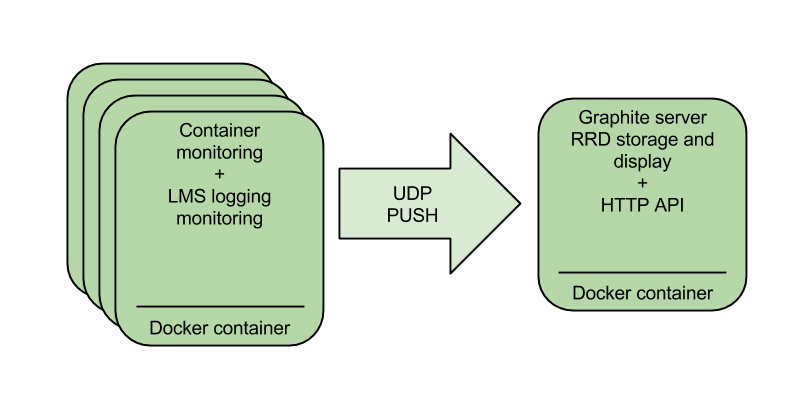
\includegraphics[width=0.9\textwidth]{./images/mlap.png}
\caption{Monitoring layer architecture proposal}
\label{F:MLAP}
\end{center}
\end{figure}

\subsection{Application layer}\label{B:appLayerCH2}

This subsection aims to compile the minimum requirements that the core service (i.e.: the LiveMediaStreamer framework) should implement to fit within the platform. This means assuring that it can be demonstrated as an efficient real-time cloud production platform, as a prototype.

First of all, let us identify the main goals that LiveMediaStreamer framework should provide:

\begin{itemize}
	\item To assure minimal performance cost in computational terms when measuring internal metrics in order to not interfere on the overall performance of the framework, whatever the scenario setup.
	\item To calculate specific metrics of interest. Common metrics should be:
	\begin{itemize}
		\item For network usage statistics
		\begin{itemize}
			\item Bandwidth usage per incoming and outgoing streams
			\item Packet loss ratio per incoming and outgoing streams
			\item Delay variation per incoming and outgoing streams
			\item Delay from far-end clients to LMS per incoming and outgoing streams
		\end{itemize}
		\item For media statistics
		\begin{itemize}
			\item Pipeline losses 
			\item Pipeline delay  
		\end{itemize}
	\end{itemize}
	\item To compile the metrics in an efficient manner in order to let them be gathered by Collectd or any other application.
\end{itemize}

Currently, as of revision 0.2, the LiveMediaStreamer framework does not implement any metrics gathering neither logging.

Regarding network usage statistics, LiveMediaStreamer does not support any internal metrics gathering at network modules (i.e.: receiver and transmitter) where the Live555 library is implemented. However, the Live555 library allows a quick implementation of network statistics measurements (i.e.: bandwidth, losses, jitter, delay). 

Thanks to Live555 examples (i.e.: the testProgs folder inside the source code library path) it becomes easy to understand how to gather network statistics at the input side. But, regarding output network statistics, it is not so obvious which is the optimal solution. This fact is mainly due to having two options which imply to implement the metrics gathering by doing some methods' re-implementation of the RTP (i.e.: first option) or the RTCP (i.e.: second option) main classes, but this specific problem statement will be treated in Chapter \ref{D:application}.

Regarding media statistics, current LiveMediaStreamers' version of the framework does not implement any metrics gathering. So, in order to minimize computational cost of such measurements we propose to implement:

\begin{itemize}
\item A specific method to measure processing delays (i.e.: the time a frame takes to be processed within a path).
\item A specific method to measure processing losses.
\end{itemize}

Then, in order to implement the metrics presentation to be logged for external applications, a middleware API is required to be developed. Current API is not at all an API but a web GUI API for an specific scenario (i.e.: AVMixer scenario, as mentioned in Chapter \ref{A:stateOfTheArt} Section \ref{SOA:LMS}), which means that it is required to implement a more generic middleware API to let external applications to log the LMS internal metrics as API definition reclaims. Therefore, the proposal for solving this issue is to develop a RESTfull API in order to present the metrics from the LMS instance. This implementation is an opportunity to develop a full API for managing the LiveMediaStreamer framework over HTTP.  Moreover, such middleware will ease to develop new applications over the LMS framework by evolving it as a SaaS, which means a proper enhancement to fit in a cloud environment. 

\begin{figure}[htb]
\begin{center}
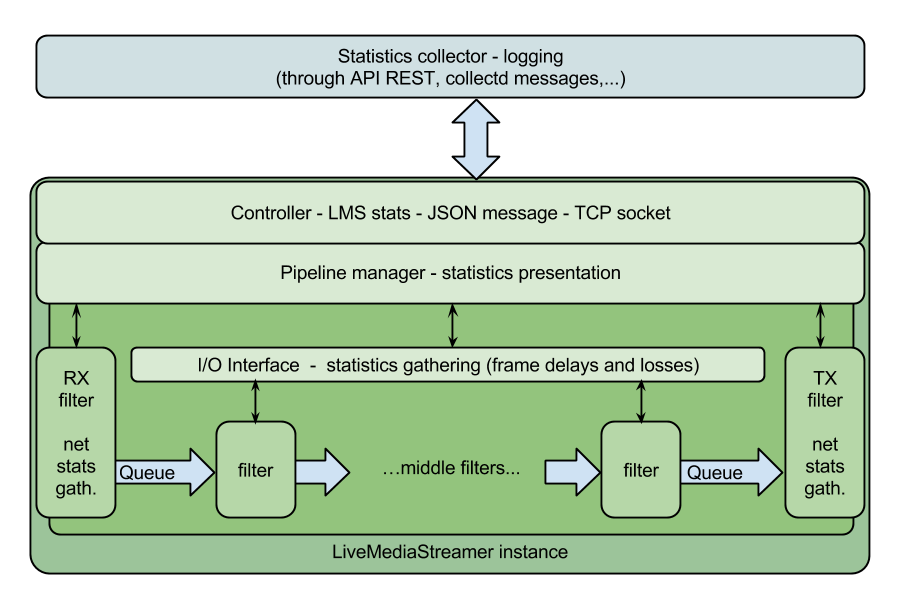
\includegraphics[width=0.95\textwidth]{./images/appArch.png}
\caption{LiveMediaStreamer framework statistics gathering and logging proposal}
\label{F:appArch}
\end{center}
\end{figure}

Figure \ref{F:appArch} illustrates how previous statements are proposed to be implemented. As it can be seen in Appendix \ref{ANX:lmsarchfull}, each filter can have one or more readers and writers (both are inheritors of the IOInterface class). This issue will be described in Chapter \ref{D:application}.

Finally, the Pipelinemanager class instance is the class responsible for compiling the metrics, filter by filter, when they are requested by the Controller class instance. 

\section{Architecture proposal}

Once the problem statement has been described for each defined layer (i.e.: virtualization, monitoring and application) of the platform, a global architecture can be proposed. This is shown in Figure \ref{F:overallArchProp} which tries to be as generic as possible in order to illustrate the possibilities of the platform. There are different physical servers shown in order to demonstrate the aim to also support flexibility and scalability. In the following chapters (specifically the conclusions Chapter \ref{H:platformDeploymentAndDemonstrations}) we will demonstrate the feasibility of the approach. 

\begin{figure}[!htb]
\begin{center}
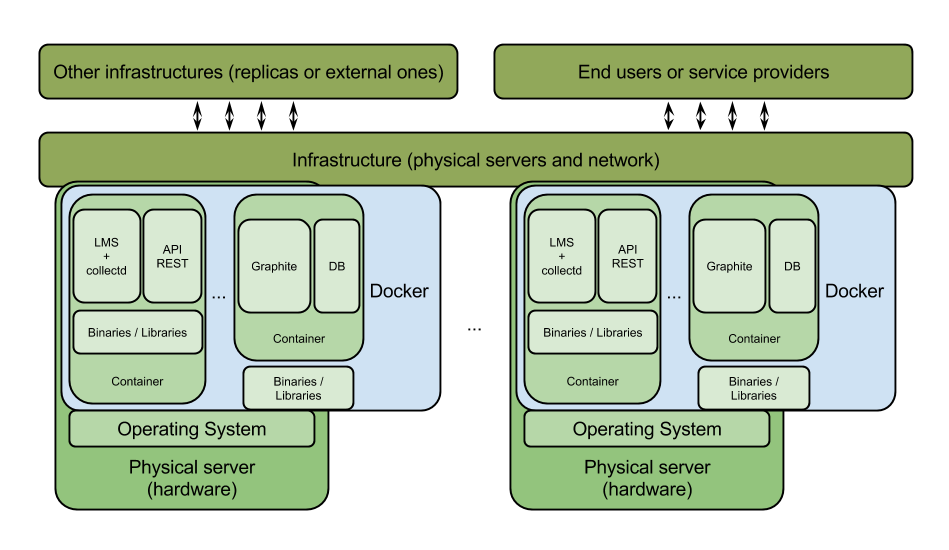
\includegraphics[width=0.95\textwidth]{./images/overallArchProp.png}
\caption{Proposal of the platform architecture}
\label{F:overallArchProp}
\end{center}
\end{figure}


Moreover, each physical server has different types of containers where different and possible combinations and configurations of the technologies are shown that might be deployed and used for specific use cases (scenarios).

\begin{figure}[!htb]
\begin{center}
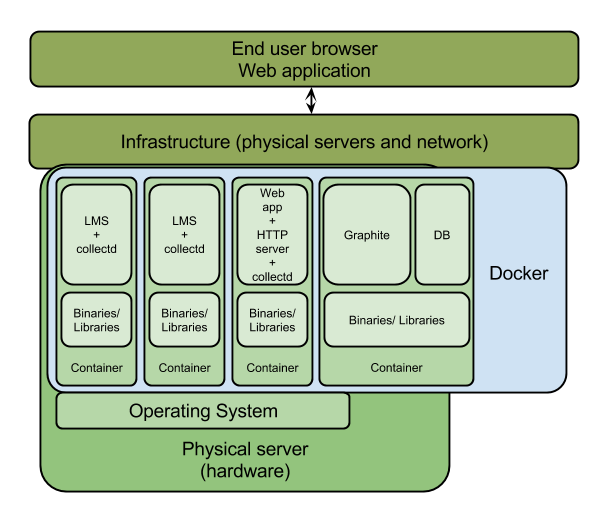
\includegraphics[width=0.7\textwidth]{./images/exampleArch.png}
\caption{Example of specific platform deployment}
\label{F:exampleArch}
\end{center}
\end{figure} 

For example, a possible and specific architecture configuration could be a transcoder scenario. Figure \ref{F:exampleArch} shows a simple example of a transcoding service behind a web application. This use case includes an user, which configures and manages the LiveMediaStreamer's scenario configured for a transcoding service (e.g.: starting with a HTML input form for incoming inputs, transcoding parameters and RTSP server configuration). Specifically, at the architecture level, there is a container with an LMS daemon running, another one with the REST API that receives queries from the HTTP server from another container, which is serving the web application to the end user (e.g.: web browser). Then, each container has a collectd client that parses the logs of interest and sends the metrics to the Graphite service. Therefore, through the web interface the user can see specific graphics (e.g.: CPU usage, data losses, bandwidth usage, \ldots) from the graphite server (in another container) in order to monitor the overall performance and actuate if required.  

Finally, it is important to point out that what will be deployed in order to demonstrate the platform feasibility is an specific scenario, but it is as generic as possible. This will be detailed in Chapter \ref{H:platformDeploymentAndDemonstrations}.

\section{Task planning}

This section describes the tasks to be done and its precedence. 

\begin{figure}[!htb]
\begin{center}
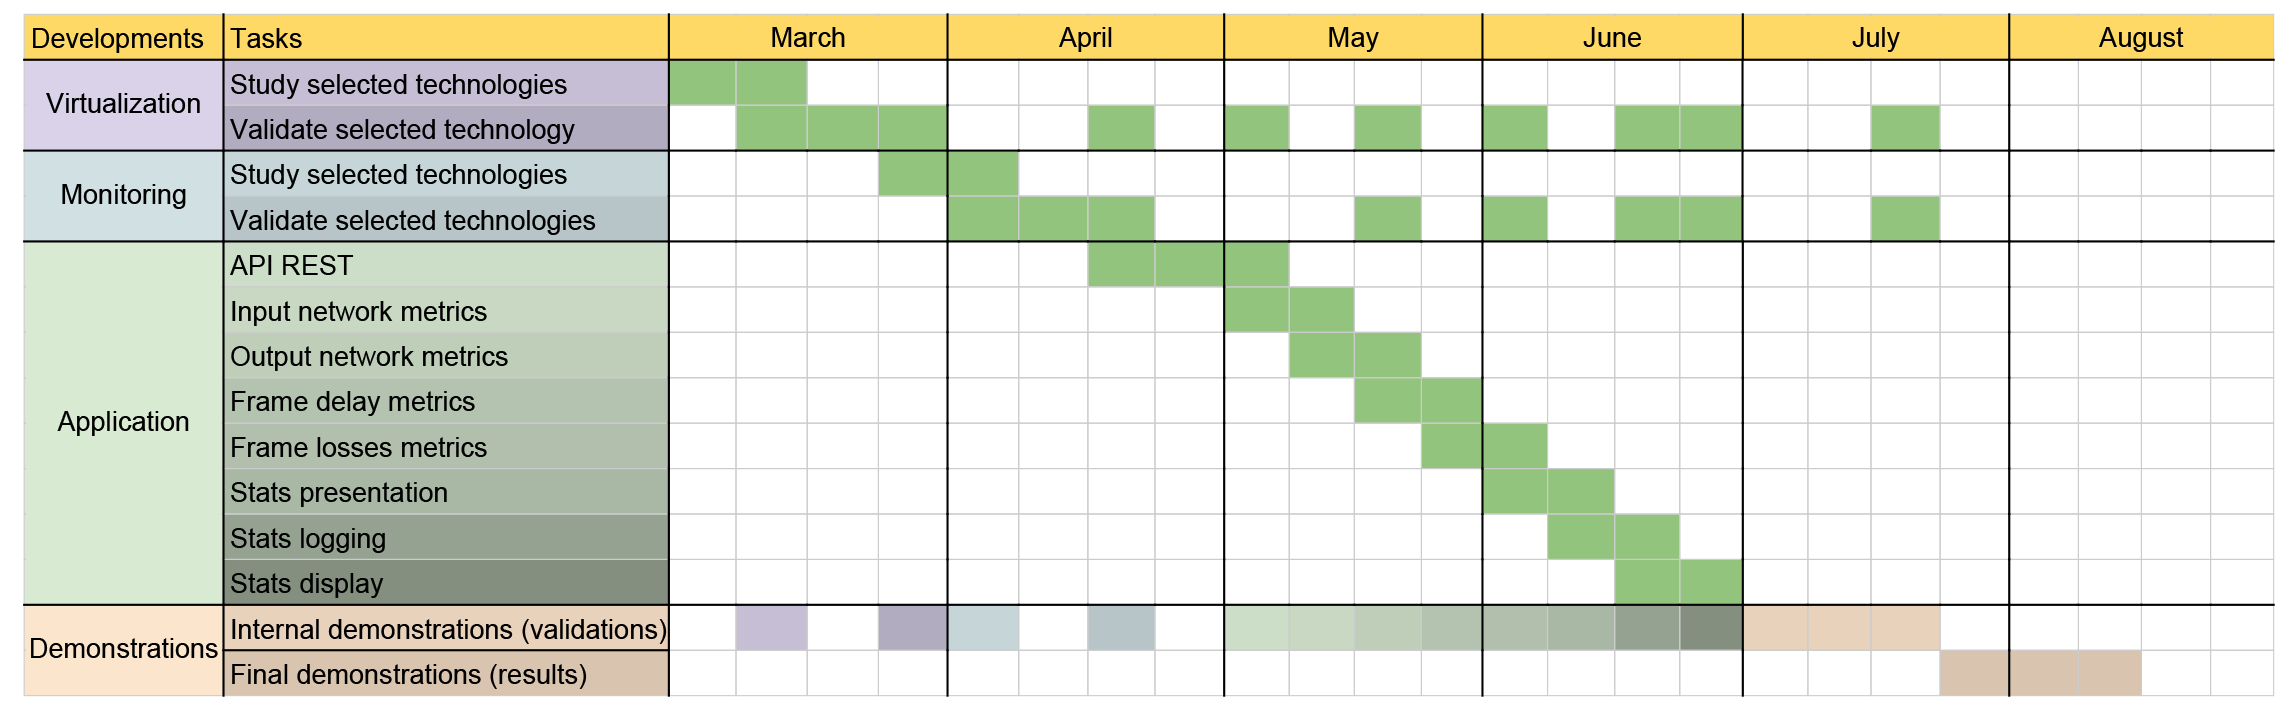
\includegraphics[width=1\textwidth]{./images/gantt.png}
\caption{Task planning - Gantt proposal}
\label{F:tpgp}
\end{center}
\end{figure}

Figure \ref{F:tpgp} is the Gantt proposal for the task planning organization. It takes into account a period of six months for the execution of this thesis and it shows specific periods per task. For example, some tasks might seem overloaded, but this is taking into account that the whole time will not be spent on working in the thesis but other tasks related to tasks carried out at the i2CAT Foundation.

Note that the fact of working with a team inside an organization means extra tasks such as internal demonstrations periods in order to carry out specific validations. 

The following chapters describes the work done in each one of the topics: Application (Chapter \ref{D:application}), virtualization (Chapter \ref{D:virtualization}), monitoring (Chapter \ref{G:monitoringLayer}) and testing and deployment (Chapter \ref{H:platformDeploymentAndDemonstrations}). 
